% Options for packages loaded elsewhere
\PassOptionsToPackage{unicode}{hyperref}
\PassOptionsToPackage{hyphens}{url}
%
\documentclass[
]{article}
\usepackage{amsmath,amssymb}
\usepackage{lmodern}
\usepackage{iftex}
\ifPDFTeX
  \usepackage[T1]{fontenc}
  \usepackage[utf8]{inputenc}
  \usepackage{textcomp} % provide euro and other symbols
\else % if luatex or xetex
  \usepackage{unicode-math}
  \defaultfontfeatures{Scale=MatchLowercase}
  \defaultfontfeatures[\rmfamily]{Ligatures=TeX,Scale=1}
\fi
% Use upquote if available, for straight quotes in verbatim environments
\IfFileExists{upquote.sty}{\usepackage{upquote}}{}
\IfFileExists{microtype.sty}{% use microtype if available
  \usepackage[]{microtype}
  \UseMicrotypeSet[protrusion]{basicmath} % disable protrusion for tt fonts
}{}
\makeatletter
\@ifundefined{KOMAClassName}{% if non-KOMA class
  \IfFileExists{parskip.sty}{%
    \usepackage{parskip}
  }{% else
    \setlength{\parindent}{0pt}
    \setlength{\parskip}{6pt plus 2pt minus 1pt}}
}{% if KOMA class
  \KOMAoptions{parskip=half}}
\makeatother
\usepackage{xcolor}
\usepackage[margin=1in]{geometry}
\usepackage{graphicx}
\makeatletter
\def\maxwidth{\ifdim\Gin@nat@width>\linewidth\linewidth\else\Gin@nat@width\fi}
\def\maxheight{\ifdim\Gin@nat@height>\textheight\textheight\else\Gin@nat@height\fi}
\makeatother
% Scale images if necessary, so that they will not overflow the page
% margins by default, and it is still possible to overwrite the defaults
% using explicit options in \includegraphics[width, height, ...]{}
\setkeys{Gin}{width=\maxwidth,height=\maxheight,keepaspectratio}
% Set default figure placement to htbp
\makeatletter
\def\fps@figure{htbp}
\makeatother
\setlength{\emergencystretch}{3em} % prevent overfull lines
\providecommand{\tightlist}{%
  \setlength{\itemsep}{0pt}\setlength{\parskip}{0pt}}
\setcounter{secnumdepth}{-\maxdimen} % remove section numbering
\newlength{\cslhangindent}
\setlength{\cslhangindent}{1.5em}
\newlength{\csllabelwidth}
\setlength{\csllabelwidth}{3em}
\newlength{\cslentryspacingunit} % times entry-spacing
\setlength{\cslentryspacingunit}{\parskip}
\newenvironment{CSLReferences}[2] % #1 hanging-ident, #2 entry spacing
 {% don't indent paragraphs
  \setlength{\parindent}{0pt}
  % turn on hanging indent if param 1 is 1
  \ifodd #1
  \let\oldpar\par
  \def\par{\hangindent=\cslhangindent\oldpar}
  \fi
  % set entry spacing
  \setlength{\parskip}{#2\cslentryspacingunit}
 }%
 {}
\usepackage{calc}
\newcommand{\CSLBlock}[1]{#1\hfill\break}
\newcommand{\CSLLeftMargin}[1]{\parbox[t]{\csllabelwidth}{#1}}
\newcommand{\CSLRightInline}[1]{\parbox[t]{\linewidth - \csllabelwidth}{#1}\break}
\newcommand{\CSLIndent}[1]{\hspace{\cslhangindent}#1}
\usepackage{setspace}
\doublespacing
\usepackage{lineno}
\linenumbers
\ifLuaTeX
  \usepackage{selnolig}  % disable illegal ligatures
\fi
\IfFileExists{bookmark.sty}{\usepackage{bookmark}}{\usepackage{hyperref}}
\IfFileExists{xurl.sty}{\usepackage{xurl}}{} % add URL line breaks if available
\urlstyle{same} % disable monospaced font for URLs
\hypersetup{
  hidelinks,
  pdfcreator={LaTeX via pandoc}}

\author{}
\date{\vspace{-2.5em}}

\begin{document}

\hypertarget{character-displacement-of-bill-ratio-in-penguins}{%
\section{Character displacement of bill ratio in
penguins}\label{character-displacement-of-bill-ratio-in-penguins}}

Lucas Eckert\textsuperscript{1*}

\begin{enumerate}
\def\labelenumi{\arabic{enumi}.}
\tightlist
\item
  Department of Biology, McGill University, Montreal, QC, Canada
\end{enumerate}

*Corresponding Author

Email: lucas.eckert@mail.mcgill.ca

\hypertarget{abstract}{%
\section{Abstract}\label{abstract}}

\hypertarget{introduction}{%
\section{Introduction}\label{introduction}}

Character displacement in Darwin's finches (Grant \& Grant 2006).

\hypertarget{methods}{%
\section{Methods}\label{methods}}

The bill ratio was defined as follows:

\[
BillRatio = BillDepth \div BillLength
\]

We used R version 4.2.2 (R Core Team 2022) and the following R packages:
GGally v. 2.1.2 (Schloerke \emph{et al.} 2021), palmerpenguins v. 0.1.1
(Horst \emph{et al.} 2020), rmarkdown v. 2.18 (Xie \emph{et al.} 2018,
2020; Allaire \emph{et al.} 2022), tidyverse v. 1.3.2 (Wickham \emph{et
al.} 2019).

\hypertarget{results}{%
\section{Results}\label{results}}

As expected, there is a positive relationship between bill length and
depth in all three species of penguins (Figure 1).

\begin{figure}
\centering
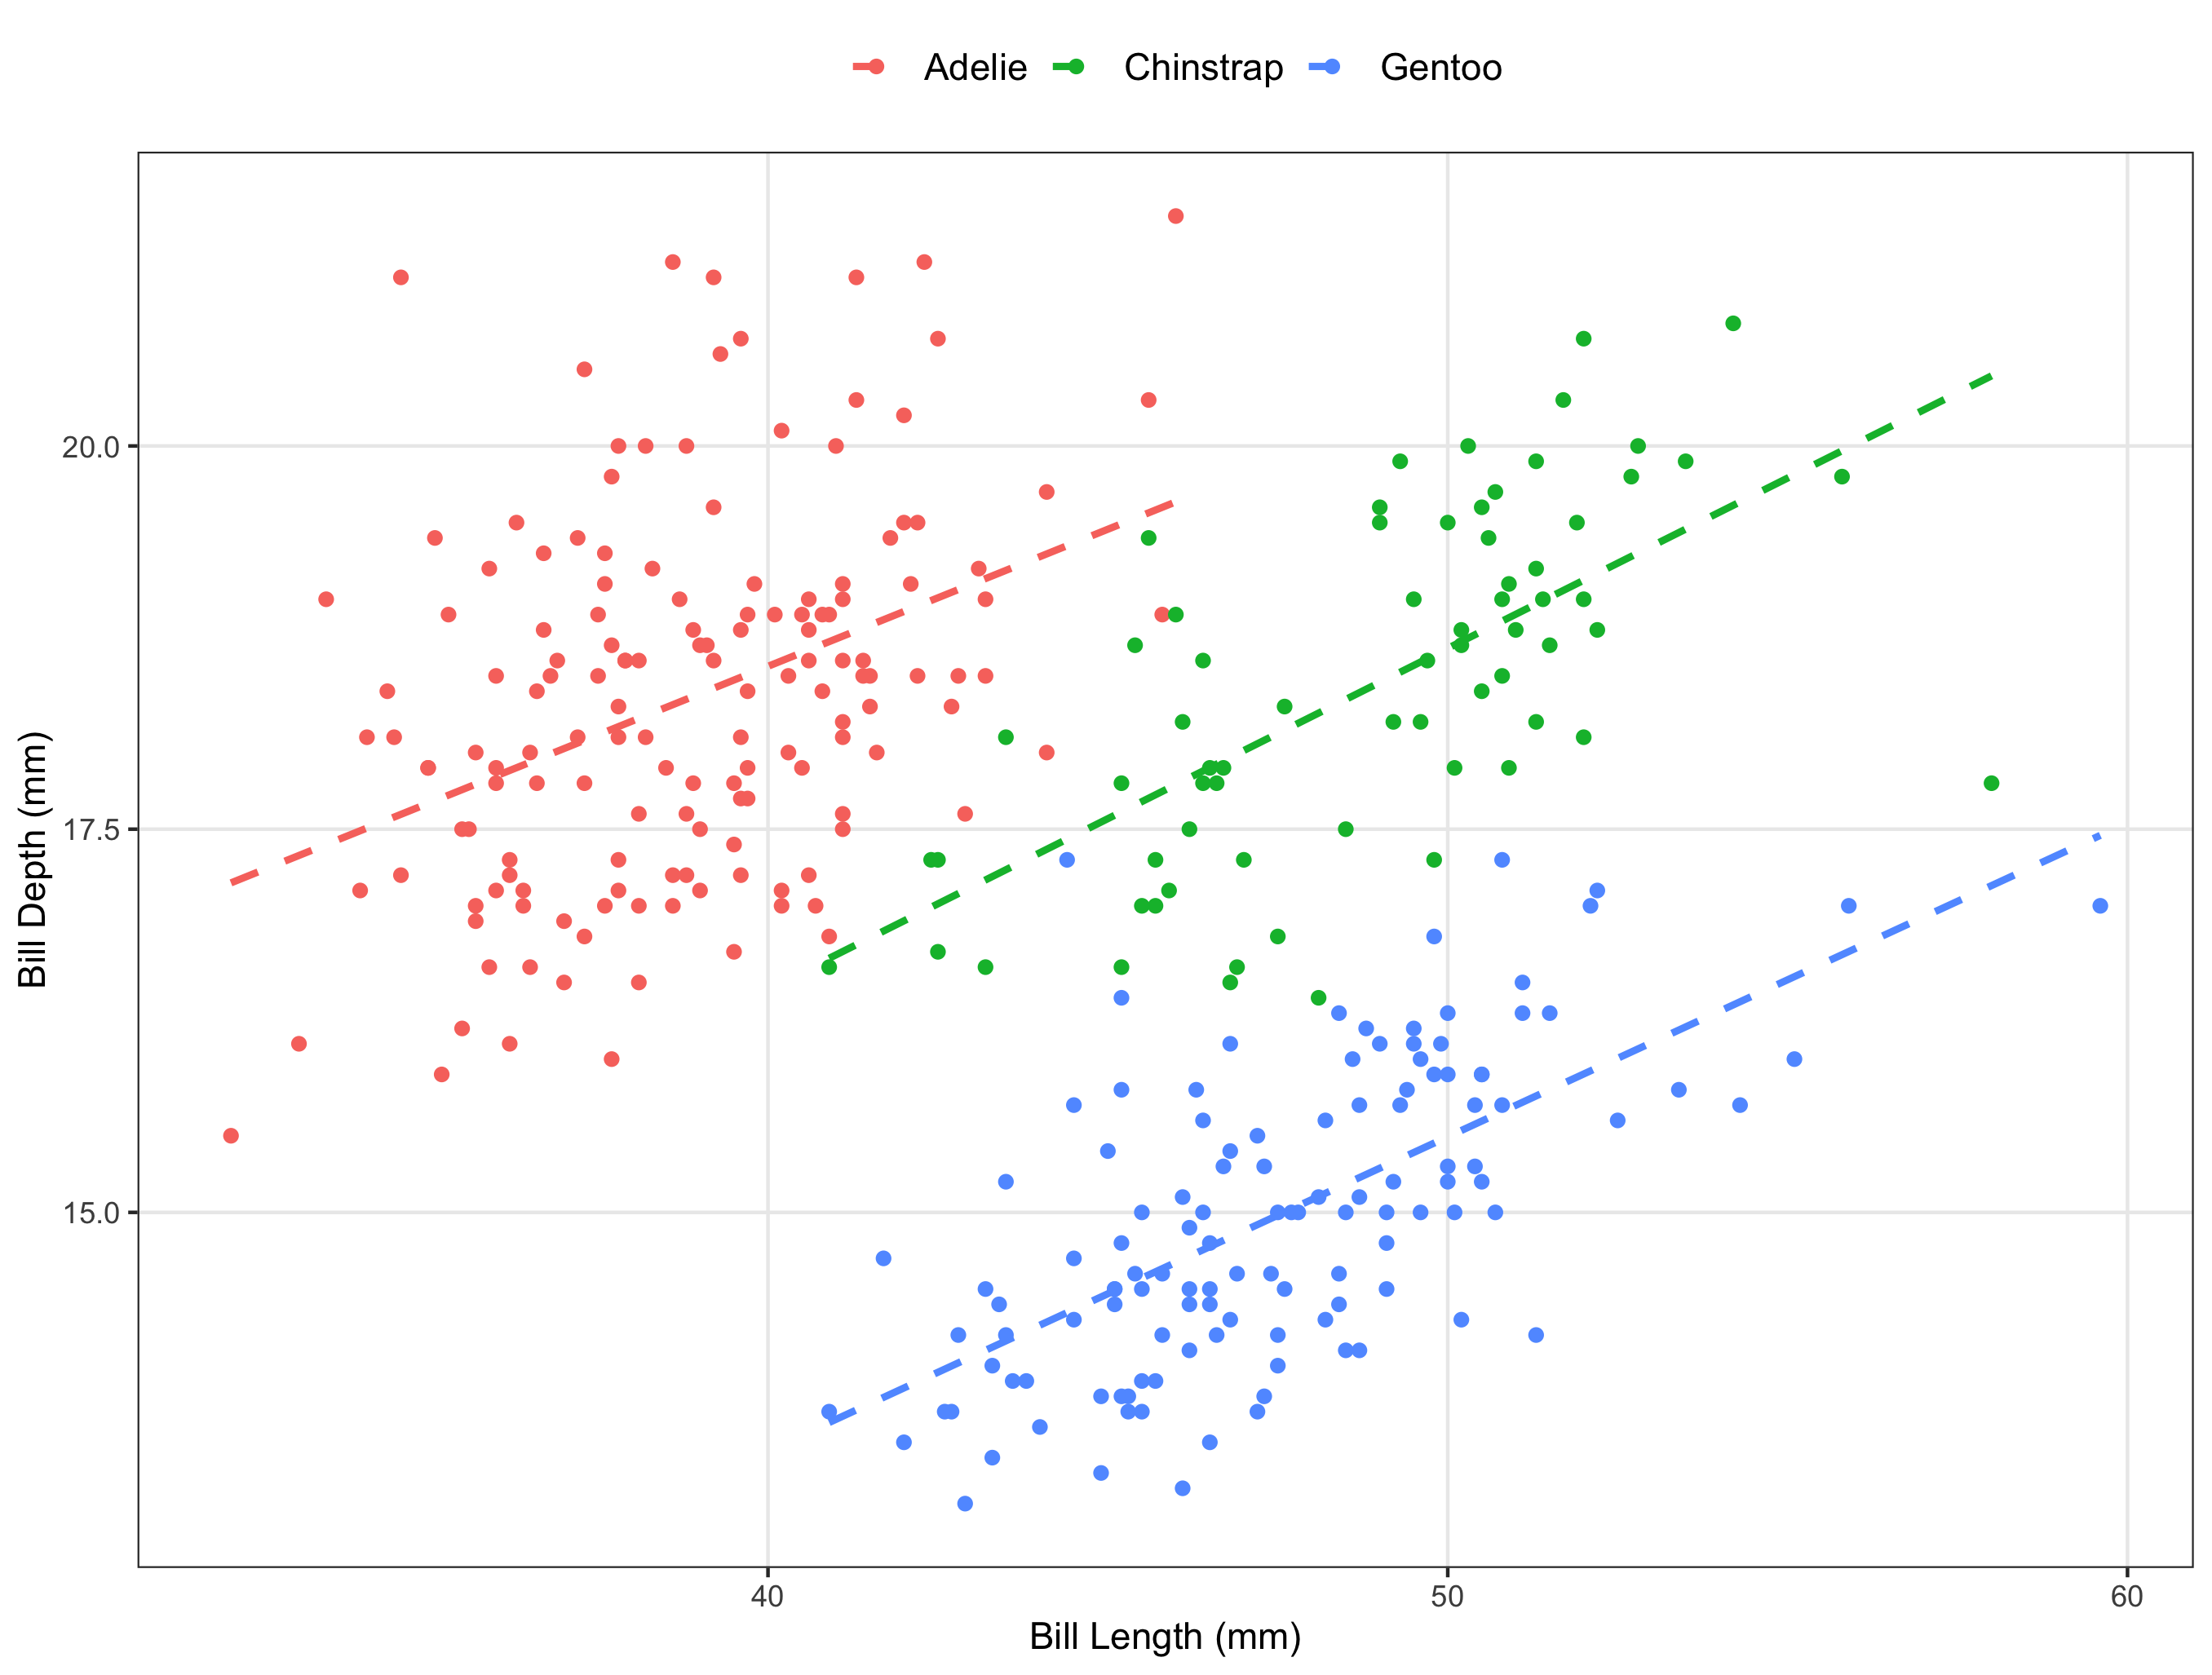
\includegraphics{images/figure1.png}
\caption{Figure 1: Positive relationship between bill length and depth
(both in mm) for each species.}
\end{figure}

The species also differ in mean bill ratio (Figure 2). Adelie penguins
have the greatest bill ratio (mean = 0.474), followed by Chinstrap (mean
= 0.378), then Gentoo (mean = 0.316). Significant differences were
confirmed among all three species using pairwise T-tests.

\begin{figure}
\centering
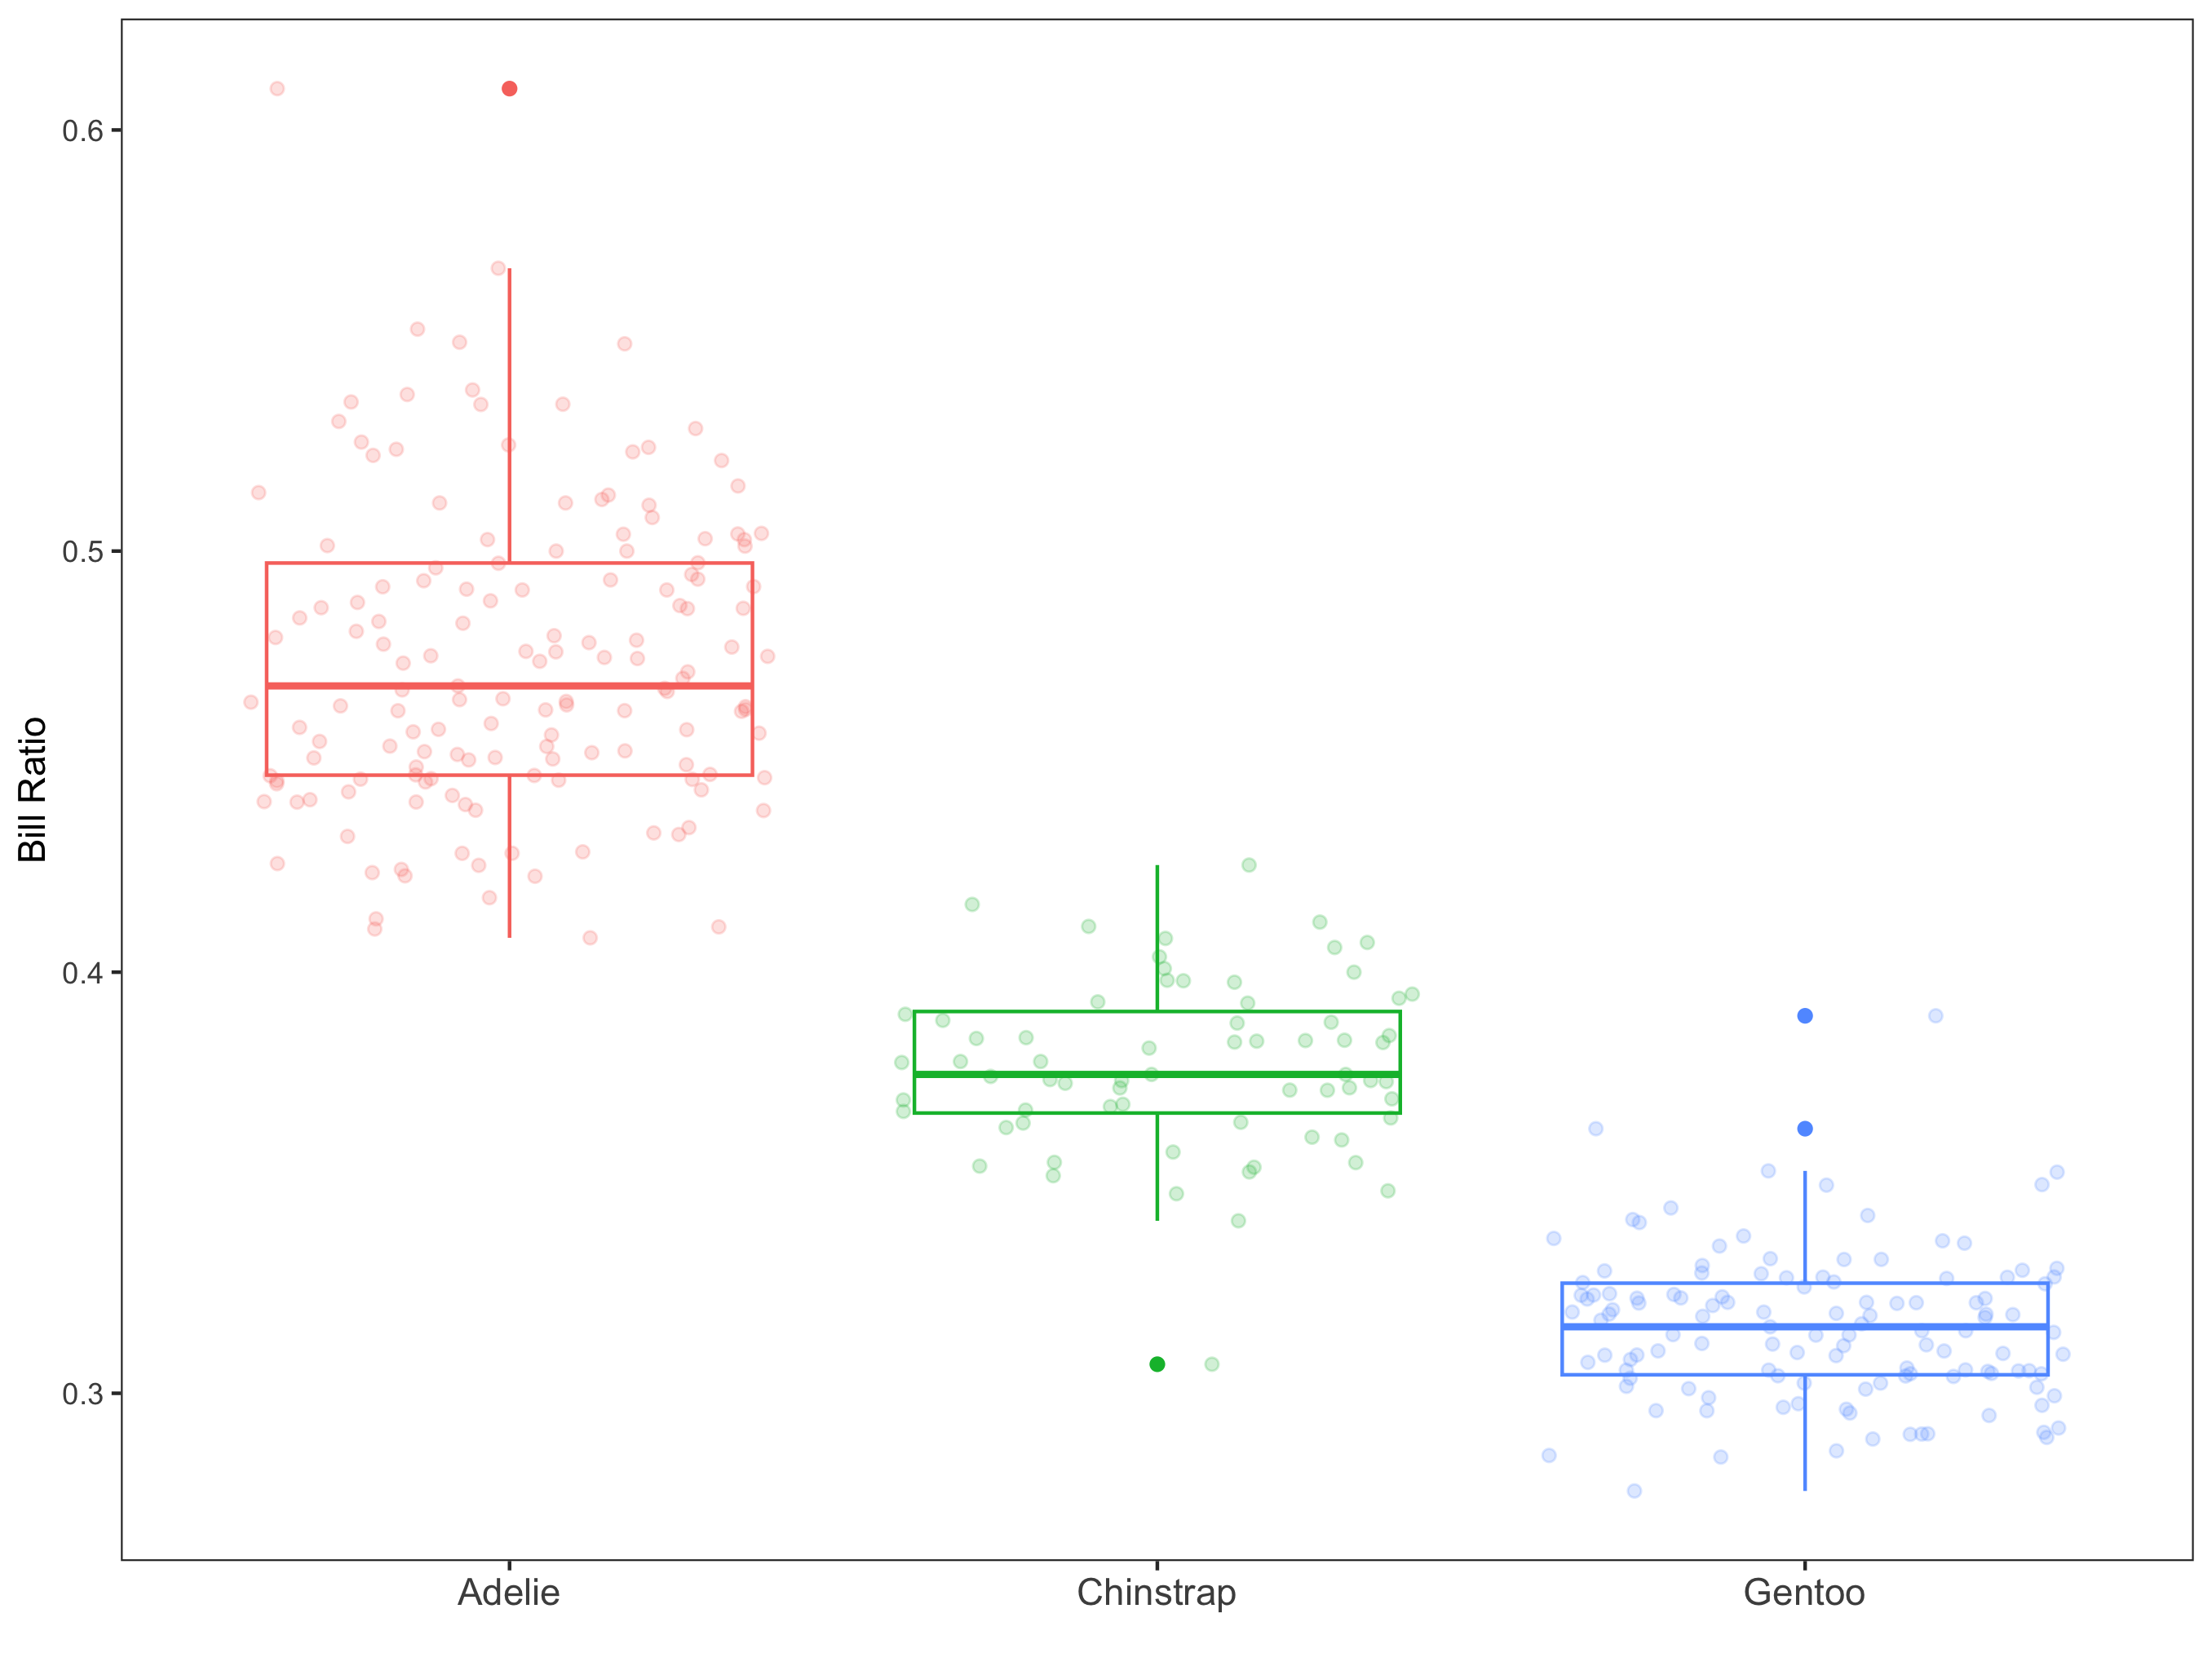
\includegraphics{images/figure2.png}
\caption{Figure 2: Comparison of bill ratio among species.}
\end{figure}

\hypertarget{discussion}{%
\section{Discussion}\label{discussion}}

\hypertarget{references}{%
\section*{References}\label{references}}
\addcontentsline{toc}{section}{References}

\hypertarget{refs}{}
\begin{CSLReferences}{1}{0}
\leavevmode\vadjust pre{\hypertarget{ref-rmarkdown2022}{}}%
Allaire, J., Xie, Y., McPherson, J., Luraschi, J., Ushey, K., Atkins,
A., \emph{et al.} (2022).
\emph{\href{https://github.com/rstudio/rmarkdown}{{rmarkdown}: Dynamic
documents for r}}.

\leavevmode\vadjust pre{\hypertarget{ref-grant2006}{}}%
Grant, P.R. \& Grant, B.R. (2006).
\href{https://doi.org/10.1126/science.1128374}{Evolution of character
displacement in darwin's finches}. \emph{Science}, 313, 224--226.

\leavevmode\vadjust pre{\hypertarget{ref-palmerpenguins}{}}%
Horst, A.M., Hill, A.P. \& Gorman, K.B. (2020).
\emph{\href{https://doi.org/10.5281/zenodo.3960218}{{palmerpenguins}:
Palmer archipelago (antarctica) penguin data}}.

\leavevmode\vadjust pre{\hypertarget{ref-base}{}}%
R Core Team. (2022). \emph{\href{https://www.R-project.org/}{{R}: A
language and environment for statistical computing}}. R Foundation for
Statistical Computing, Vienna, Austria.

\leavevmode\vadjust pre{\hypertarget{ref-GGally}{}}%
Schloerke, B., Cook, D., Larmarange, J., Briatte, F., Marbach, M.,
Thoen, E., \emph{et al.} (2021).
\emph{\href{https://CRAN.R-project.org/package=GGally}{{GGally}:
Extension to {``{ggplot2}''}}}.

\leavevmode\vadjust pre{\hypertarget{ref-tidyverse}{}}%
Wickham, H., Averick, M., Bryan, J., Chang, W., McGowan, L.D., François,
R., \emph{et al.} (2019).
\href{https://doi.org/10.21105/joss.01686}{Welcome to the {tidyverse}}.
\emph{Journal of Open Source Software}, 4, 1686.

\leavevmode\vadjust pre{\hypertarget{ref-rmarkdown2018}{}}%
Xie, Y., Allaire, J.J. \& Grolemund, G. (2018).
\emph{\href{https://bookdown.org/yihui/rmarkdown}{R markdown: The
definitive guide}}. Chapman; Hall/CRC, Boca Raton, Florida.

\leavevmode\vadjust pre{\hypertarget{ref-rmarkdown2020}{}}%
Xie, Y., Dervieux, C. \& Riederer, E. (2020).
\emph{\href{https://bookdown.org/yihui/rmarkdown-cookbook}{R markdown
cookbook}}. Chapman; Hall/CRC, Boca Raton, Florida.

\end{CSLReferences}

\end{document}
